\documentclass{article}

\setlength{\topmargin}{-.5in}
\setlength{\oddsidemargin}{.0in}
\setlength{\evensidemargin}{.0in}
\setlength{\textheight}{9in}
\setlength{\textwidth}{6.5in}
\setlength{\parindent}{0in}
%\parskip=.125in

\usepackage{amsmath,bm}%
\usepackage{amsfonts}%
\usepackage{enumerate}%

\newcommand{\beaa}{\begin{eqnarray*}}
\newcommand{\eeaa}{\end{eqnarray*}}
\newcommand{\bea}{\begin{eqnarray}}
\newcommand{\eea}{\end{eqnarray}}
\newcommand{\svskip}{\vspace{.2in}}
\newcommand{\mvskip}{\vspace{.25in}}
\newcommand{\lvskip}{\vspace{.5in}}
\def\E{\mathop{\rm E\,}\nolimits}
\def\Var{\mathop{\rm Var\,}\nolimits}
\def\Cov{\mathop{\rm Cov\,}\nolimits}
\def\Cor{\mathop{\rm Corr\,}\nolimits}
\def\Tr{\mathop{\rm Tr\,}\nolimits}
\def\diag{\mathop{\rm diag\,}\nolimits}
\def\midd{\mathop{\,|\,}\nolimits}
\def\cip{\mathop{\stackrel{P}{\rightarrow}}\nolimits}
\def\cid{\mathop{\stackrel{d}{\rightarrow}}\nolimits}
\def\ciqm{\mathop{\stackrel{\mbox{\scriptsize qm}}{\rightarrow}}\nolimits}
\def\defn{{\stackrel{\mbox{\scriptsize def}}{=}}}
\def\eid{{\stackrel{{\cal D}}{=}}}
\def\rvseq{\mathop{X_1, X_2, \ldots}\nolimits}
\def\rvseqn{\mathop{X_1, \ldots, X_n}\nolimits}
\def\u#1{{\underline{#1}}}
\def\o#1{{\overline{#1}}}
\def\n#1{^{(#1)}}
\newcommand{\qed}{\rule{2mm}{2mm}}


\def\cas{\mathop{\stackrel{\mbox{\scriptsize as}}{\rightarrow}}\nolimits}

\pagestyle{empty}

%%-------------------------------------------------------------------

\usepackage{Sweave}
\begin{document}
        \hrule
        \begin{center}
        \Large\bf Stat 515: Stochastic Processes I \hfill Spring 2012\\
        Take-Home Final Exam  \hfill April 21--May 2, 2012
        \end{center}
        \hrule

%\lvskip {\bf Name:  \rule{4in}{.01in}}

\mvskip 
This exam is worth 10 points.  You have 11 days.  Electronic submission
is required.  {\em Show all of your work for full credit; answers submitted without
supporting work will receive little or no credit.}  
The rules of the exam are as follows:

\begin{enumerate}
\item[A.]
You may not communicate about this exam with anyone other than the instructor, not even the grader. You may not receive help of any kind on this exam from anyone else except the instructor. You may not give help of any kind on this exam to anyone else.
\item [B.]
You must submit your writeup and your code to ANGEL, in the appropriate dropboxes, before 5:00pm on Wednesday, May 2.  Do not include your code in your writeup; the code must be easy to read (with comments as appropriate) and it should be clear how I can run it.  You may use R, Matlab, or Python.  I strongly encourage the use of a sensible text editor in preparing your code.
\end{enumerate}



\lvskip 
{\bf Problem 1. [2 points]\ } 
Suppose that a player has five dollars and wishes to play craps until she either runs out of money or 
doubles her money (i.e., until the first time she has either zero dollars or some amount greater than
or equal to ten dollars), at which point she stops playing.   
Betting in craps works as follows:  If the player has $x$ dollars and
bets $y$ dollars (where $y\le x$), then 
with probability $244/495$, she wins and her new total is $x+y$; with probability
$251/495$, she loses and her new total is $x-y$.

\svskip
{\bf(a) \ }
Suppose that the player always bets one dollar.  What is the probability that she will eventually
double her money?
\begin{quotation}{\bf Solution:}
This is an example of Gambler's ruin.  With $p=244/495$, the probability
of getting to 10 before 0 if you start from 5 is
\[
\frac{1 - \left( \frac{251}{244} \right)^5 }{1 - \left( \frac{251}{244} \right)^{10}} = 0.4647
\]
\end{quotation}

\svskip
{\bf(b) \ }
Suppose that for each new game, the player bets $3$, $2$, or $1$ dollar with probabilities
$1/6$, $2/6$, and $3/6$, respectively.  (If she only has two dollars left, she bets $2$ or $1$ dollar
with probabilities $1/3$ and $2/3$, respectively.  If she only has one dollar left, she bets one 
dollar.)  
What is the expected number of games she will be able to play before stopping
(at either zero dollars or ten or more dollars)?
\begin{quotation}{\bf Solution:}
If we make 0 and 10 absorbing states, and $p=1-q=244/495$, then the transition probability
matrix for the Markov chain in which her current wealth is the state equals
\setcounter{MaxMatrixCols}{12}
\[
P = \begin{bmatrix}
1 & 0 & 0 & 0 & 0 & 0 & 0 & 0 & 0 & 0 & 0 \cr
q & 0 & p & 0 & 0 & 0 & 0 & 0 & 0 & 0  & 0 \cr
q/3&2q/3&0&2p/3&p/3&0& 0 & 0 & 0 & 0 & 0 \cr
q/6&q/3&q/2&0&p/2&p/3&p/6& 0 & 0 & 0 & 0 \cr
0 & q/6&q/3&q/2&0&p/2&p/3&p/6& 0 & 0 & 0  \cr
0 & 0 & q/6&q/3&q/2&0&p/2&p/3&p/6& 0 & 0  \cr
0 & 0 & 0 & q/6&q/3&q/2&0&p/2&p/3&p/6& 0   \cr
0 & 0 & 0 & 0 & q/6&q/3&q/2&0&p/2&p/3&p/6  \cr
0 & 0 & 0 & 0 & 0 & q/6&q/3&q/2&0&p/2&p/2  \cr
0 & 0 & 0 & 0 & 0 & 0 & q/6&q/3&q/2&0&p   \cr
0 & 0 & 0 & 0 & 0 & 0 & 0 & 0 & 0 & 0 & 1 \cr
\end{bmatrix}
\]
To find the expected time spent in states 1 through 9, we look at  
$S=(I-P_T)^{-1}$, where $P_T$ is the $9\times9$ submatrix of $P$ corresponding to 
states 1 through 9.  The answer we are after is the sum of the whole 5th row of $S$:
\begin{Schunk}
\begin{Sinput}
> Pt=rbind( c(0, 6, 0, 0, 0, 0, 0, 0, 0),
+                 c(4, 0, 4, 2, 0, 0, 0, 0, 0),
+                 c(2, 3, 0, 3, 2, 1, 0, 0, 0),
+                 c(1, 2, 3, 0, 3, 2, 1, 0, 0),
+                 c(0, 1, 2, 3, 0, 3, 2, 1, 0),
+                 c(0, 0, 1, 2, 3, 0, 3, 2, 1),
+                 c(0, 0, 0, 1, 2, 3, 0, 3, 2),
+                 c(0, 0, 0, 0, 1, 2, 3, 0, 3),
+                 c(0, 0, 0, 0, 0, 1, 2, 3, 0)) / 6
> Pt[row(Pt)<col(Pt)] <- Pt[row(Pt)<col(Pt)] * 244/495
> Pt[row(Pt)>col(Pt)] <- Pt[row(Pt)>col(Pt)] * 251/495
> S <- solve(diag(rep(1,9)) - Pt)
> sum(S[5,])
\end{Sinput}
\begin{Soutput}
[1] 8.948682
\end{Soutput}
\end{Schunk}
We conclude that the expected number of games is 8.95.
\end{quotation}


\mvskip
{\bf Problem 2. [8 points]\ }
Suppose we have parameters distributed as follows:
\begin{eqnarray*}
\theta_0, \theta_1 & \stackrel{\rm iid}{\sim} & N(0,1),\\
\lambda  &\sim& \mbox{beta}(2,2), 
\quad\mbox{independently of $\theta_0$ and $\theta_1$.}\\ 
\end{eqnarray*}
Furthermore, suppose that, conditional on the parameters,
\begin{eqnarray*}
Z_1, \ldots, Z_{10} & \stackrel{\rm iid}{\sim} & \mbox{Bernoulli}(\lambda). \\
\end{eqnarray*}
(In other words, $P(Z_i=1) = 1-P(Z_i=0) = \lambda$.)
Finally, assume that $X_1, \ldots, X_{10}$ are conditionally independent---conditional 
on the parameters and the $Z_i$---with mass function
\[
p(x_i \mid Z_i, \theta_0, \theta_1, \lambda) =
{{20} \choose x_i }
\left( \frac{e^{x_i \theta_0}}{(1 + e^{\theta_0)^{20}}} \right)^{1-Z_i}
\left( \frac{e^{x_i \theta_1}}{(1 + e^{\theta_1})^{20}} \right)^{Z_i}
\quad\mbox{for $i=1, \ldots, 10$.}
\]
Intuitively, this means that
$X_i$ is conditionally distributed as 
binomial$(20, p_i)$, where 
%binomial$(20, \exp\{\theta_{Z_i} \} / (1+\exp\{\theta_{Z_i} \} )$, where 
\[
p_i = \frac{\exp\{\theta_{Z_i}\}}{1+\exp\{\theta_{Z_i}\}}.
\]

\svskip
{\bf (a) [4 points]\ }
Here are the data:

\svskip
\begin{tabular}{c|cccccccccc}
$i$ & 1 & 2 & 3 & 4 & 5 & 6 & 7 & 8 & 9 & 10 \\ \hline
$X_i$ & 18 & 9 & 12 & 9 & 14 & 5 & 18 & 12 & 8 & 9 \\ \hline
$Z_i$ & 1 & 0 & 0 & 0 & 1 & 0 & 1 & 0 & 0 & 0 
\end{tabular}

\svskip
Using these data:

\begin{enumerate}[(i)]
\item Demonstrate that $\lambda$,
$\theta_0$, and $\theta_1$ are independent of one another
in the posterior distribution.
\begin{quotation}{\bf Solution:}
To find the likelihood, we need to multiply 
$p(X_i \mid Z_i, \theta_0, \theta_1, \lambda)$ times 
$p(Z_i \mid \theta_0, \theta_1, \lambda)$ to obtain
$p(X_i, Z_i \mid \theta_0, \theta_1, \lambda)$ for each $i$.
Then the likelihood times the prior joint density, which is proportional to the 
posterior joint density, may be written
\[
%{{20} \choose x_i }
%\frac{\Gamma(4)}{\Gamma(2)\Gamma(2)}
%\frac{1}{2\pi}
K
\left[ \lambda^{\sum_iZ_i} (1-\lambda)^{\sum_i(1-Z_i)} \lambda(1-\lambda) \right]
\left[ \left( \frac{\exp\{ \theta_0 \sum_{i}(1-Z_i)X_i \} }{(1 + e^{\theta_0)^{20\sum_i (1-Z_i)}}} \right) \exp\{ -\theta_0^2/2\} \right]
\left[ \left( \frac{\exp\{ \theta_1 \sum_{i} Z_i X_i \}}{(1 + e^{\theta_1})^{20\sum_i Z_i}} \right) \exp\{ -\theta_1^2/2\} \right]
\]
for a constant $K$, which may be rewritten as 
\[
K
\left[ \lambda^4 (1-\lambda)^8 \right]
\left[ \left( \frac{\exp\{ 64 \theta_0 \} }{(1 + e^{\theta_0})^{140}} \right) \exp\{ -\theta_0^2/2\} \right]
\left[ \left( \frac{\exp\{ 50 \theta_1 \}}{(1 + e^{\theta_1})^{60}} \right) \exp\{ -\theta_1^2/2\} \right].
\]
It is written in this way to show clearly that the joint posterior density factors into a function of 
$\lambda$ only times a function of $\theta_0$ only times a function of $\theta_1$ only.   This
proves that the three parameters are independent in the posterior.
\end{quotation}

\item Implement three separate importance samplers 
to estimate the posterior means
of $\theta_0$, $\theta_1$, and $\lambda$, respectively.  You may 
implement your samplers using any $q$ distributions that you think
are appropriate, but please explain what your choice is in each case.
\begin{quotation}{\bf Solution:}
Since the sample proportions for $Z=0$ and $Z=1$ are 
$64/140$ and $50/60$, respectively, let us suppose that the posterior densities
for $\theta_0$ and $\theta_1$ will be peaked at roughly 
$\log(64/76)=-0.17$ and $\log(50/10)=1.61$, respectively.  

For $\lambda$, we already see that its posterior density is $\mbox{beta}(5,9)$,
which means that the exact posterior mean equals 5/14 and we don't even
have to use importance sampling.  However,
I'll go ahead and act as though we don't know this.  Let's assume that 
the posterior density for $\lambda$ has a peak
around $3/10$, since that is the proportion of $Z_i=1$.  
For the $q$ densities, I'll select $N(-0.17, 1)$ and
$N(1.61,1)$ for $\theta_0$ and $\theta_1$ and $\mbox{beta}(1.5, 3.5)$
for $\lambda$.  (The latter has mean $1.5/5=0.3$.)

The exact normalizing
constant associated with each posterior density is not known, so we will have to use 
ratio importance sampling to estimate the posterior means.  
To be very cautious in calculating the ratios required, we could do all of the calculations on 
the logarithmic scale and then exponentiate; however, by using R's built-in density functions,
we can avoid the need for this step:
\begin{Schunk}
\begin{Sinput}
> ## First, consider theta0 (with sample size one million):
> theta0 <- rnorm(n <- 1e6, mean=-.17, sd=1)
> p0<- exp(theta0)/(1+exp(theta0))
> a0 <- theta0 * dbinom(64, 140, p0) * dnorm(theta0) / dnorm(theta0, mean=-.17, sd=1)
> b0 <- dbinom(64,140,p0) * dnorm(theta0) / dnorm(theta0, mean=-.17, sd=1)
> meanTheta0 <- (muA0 <- mean(a0)) / (muB0 <- mean(b0))
> meanTheta0
\end{Sinput}
\begin{Soutput}
[1] -0.1680111
\end{Soutput}
\begin{Sinput}
> ## Next, same thing for theta1:
> theta1 <- rnorm(n, mean=1.61, sd=1)
> p1<- exp(theta1)/(1+exp(theta1))
> a1 <- theta1 * dbinom(50, 60, p1) * dnorm(theta1) / dnorm(theta1, mean=1.61, sd=1)
> b1 <- dbinom(50, 60,p1) * dnorm(theta1) / dnorm(theta1, mean=1.61, sd=1)
> meanTheta1 <- (muA1 <- mean(a1)) / (muB1 <- mean(b1))
> meanTheta1
\end{Sinput}
\begin{Soutput}
[1] 1.472498
\end{Soutput}
\begin{Sinput}
> ## Finally, for lambda:
> lambda <- rbeta(n, 1.5, 3.5)
> a2 <- lambda * dbeta(lambda, 4, 8) * dbeta(lambda, 2, 2) / dbeta(lambda, 1.5, 3.5)
> b2 <- dbeta(lambda, 4, 8) * dbeta(lambda, 2, 2) / dbeta(lambda, 1.5, 3.5)
> meanLambda <- (muA2 <- mean(a2)) / (muB2 <- mean(b2))
> c(meanLambda, 5/14) # These values should be close!
\end{Sinput}
\begin{Soutput}
[1] 0.3573152 0.3571429
\end{Soutput}
\end{Schunk}
\end{quotation}

\item 
Based on your samplers,
give 95\% confidence intervals for each of the three true posterior
means.  Make sure that you have sampled enough to ensure that
your confidence intervals are no wider than 0.01.
\begin{quotation}{\bf Solution:}
In each case, we'll use the delta-method approximation for ratio importance sampling, 
which is given by 
      \[
      {\Var} \left( \frac{ \frac1n\sum_i A_i}{\frac1n\sum_i B_i} \right) \approx
      \frac{1}{n\mu_B^2}
      \begin{bmatrix}
      1 & \frac{-\mu_A}{\mu_B}
      \end{bmatrix}
      \begin{bmatrix}
      \sigma^2_A & \sigma_{AB} \\ \sigma_{AB} & \sigma^2_B
      \end{bmatrix}
      \begin{bmatrix}
      1 \\ \frac{-\mu_A}{\mu_B}
      \end{bmatrix}.
      \]
The 95\% intervals will be equal to the estimators (from the previous part) plus or minus
$1.96$ times the square root of the approximation above in which each parameter
($\mu_A$, $\mu_B$, and the covariance matrix) is replaced by its sample estimate:
\begin{Schunk}
\begin{Sinput}
> # For theta0:
> tmp <- c(1, -muA0 / muB0)
> var0 <- tmp %*% var(cbind(a0, b0)) %*% tmp / n / muB0^2
> meanTheta0 + c(-1.96, 1.96) * sqrt(var0)
\end{Sinput}
\begin{Soutput}
[1] -0.1684933 -0.1675290
\end{Soutput}
\begin{Sinput}
> # For theta1:
> tmp <- c(1, -muA1 / muB1)
> var1 <- tmp %*% var(cbind(a1, b1)) %*% tmp / n / muB1^2
> meanTheta1 + c(-1.96, 1.96) * sqrt(var1)
\end{Sinput}
\begin{Soutput}
[1] 1.471814 1.473182
\end{Soutput}
\begin{Sinput}
> # For lambda:
> tmp <- c(1, -muA2 / muB2)
> var2 <- tmp %*% var(cbind(a2, b2)) %*% tmp / n / muB2^2
> meanLambda + c(-1.96, 1.96) * sqrt(var2)
\end{Sinput}
\begin{Soutput}
[1] 0.3570799 0.3575506
\end{Soutput}
\end{Schunk}
In each case, the intervals are much narrower than 0.01.
\end{quotation}

\end{enumerate}

\svskip
{\bf (b) [4 points]\ }
Now, suppose that not all of the data have been observed.  We
only know the following:

\svskip
\begin{tabular}{c|cccccccccc}
$i$ & 1 & 2 & 3 & 4 & 5 & 6 & 7 & 8 & 9 & 10 \\ \hline
$X_i$ & 18 & 9 & 12 & 9 & 14 & 5 & 18 & 12 & 8 & 9 \\ \hline
$Z_i$ & 1 & 0 & 0 & 0 & 1 & ?? & ?? & ?? & ?? & ?? 
\end{tabular}

\svskip
Using these data, in which $Z_6, \ldots, Z_{10}$ may now be considered
to be parameters:

\begin{enumerate}[(i)]
\item 
Derive the full conditional densities 
(up to multiplicative constants) for $\lambda$, 
$\theta_0$, and $\theta_1$.  Also derive the full conditional 
mass function for $Z_i$, where $i$ can be any value from $6$ 
to $10$.
\begin{quotation}{\bf Solution:}
Starting from the solution to part (a)(i) and plugging in the values that are known, we obtain
as the posterior joint density function
\begin{eqnarray*}
%{{20} \choose x_i }
%\frac{\Gamma(4)}{\Gamma(2)\Gamma(2)}
%\frac{1}{2\pi}
&&
K
\left[ \lambda^{3+\sum_{i=6}^{10} Z_i} (1-\lambda)^{4+\sum_{i=6}^{10}(n-Z_i)}  \right]
\left[ \left( \frac{\exp\{ \theta_0 [30+\sum_{i=6}^{10} (1-Z_i)X_i] \} }
{(1 + e^{\theta_0)^{60+20\sum_{i=6}^{10} (1-Z_i)}}} \right) \exp\{ -\theta_0^2/2\} \right] \\
&&\times 
\left[ \left( \frac{\exp\{  \theta_1 [32 +\sum_{i=6}^{10} Z_i X_i] \}}{(1 + e^{\theta_1})^{40+20\sum_{i=6}^{10} Z_i}} \right) \exp\{ -\theta_1^2/2\} \right]
\end{eqnarray*}
\end{quotation}
We obtain the full conditionals for each of the parameters from this expression.  In particular,
$\lambda$ has a beta density, $\theta_0$ and $\theta_1$ have difficult densities with no obvious
family as in part (a), and $Z_j$ has full conditional mass function
\[
\left[ \frac{ \lambda \exp\{\theta_1 X_j\}}{ (1+\exp\{\theta_1\})^{20}} \right]^{Z_j}
\left[ \frac{ (1-\lambda) \exp\{\theta_0 X_j\}}{ (1+\exp\{\theta_0\})^{20}} \right]^{1-Z_j},
\]
which is of the form $\alpha^{Z_j}\beta^{1-Z_j}$, from which we conclude that 
$Z_j$ is Bernoulli with mean $\alpha/(\alpha+\beta)$ (as explained in part ii).

\item 
Implement a variable-at-a-time Metropolis-Hastings algorithm to sample
from the posterior distribution of 
$(\theta_0, \theta_1, \lambda)$.  Describe the proposal distributions you
use for this purpose and how you decided how long to run the chain.
For the updates of $Z_6, \ldots, Z_{10}$, use Gibbs sampling together with
the fact that for any Bernoulli variable $Y$ with mass function proportional
to $\alpha^y\beta^{1-y}$,
\[
P(Y=1) = 1-P(Y=0) = \frac{\alpha}{\alpha+\beta}.
\]
\begin{quotation}{\bf Solution:}
We may use Gibbs sampling for updating $\lambda$, then Metropolis-Hastings
for updating $\theta_0$ and $\theta_1$, then Gibbs for updating the $Z_j$.
For the M-H iterations, we can propose new $\theta_0$ and $\theta_1$ values 
from a normal distribution with variance 0 centered at the current values.
This proposal is symmetric, which means that the M-H ratio simplifies to a
Metropolis ratio.  
\begin{Schunk}
\begin{Sinput}
> # Initialization:
> x <- c(18, 9, 12, 9, 14, 5, 18, 12, 8, 9)
> z <- c(1, 0, 0, 0, 1, 0, 0, 0, 0, 0) # The last five of these are arbitrary starting values
> iterations <- 1e6
> z6toz10 <- matrix(0, 1+iterations, 5)
> theta0 <- theta1 <- rep(0, 1+iterations)
> lambda <- rep(1/2, iterations)
> for (i in 1:iterations) {
+   # Step 1:  Update lambda
+   lambda[i+1] <- rbeta(1, 1+sum(z), 11-sum(z))
+   # Step 2:  Update theta0
+   Proposal <- rnorm(1, mean=theta0[i])
+   logMHRatio <- (theta0[i]^2 - Proposal^2)/2 + 
+                           (Proposal - theta0[i]) * sum((1-z) * x) -
+                           20 * sum(1-z) * log(1 + exp(Proposal)) +
+                           20 * sum(1-z) * log(1 + exp(theta0[i]))
+   theta0[i+1] <- ifelse (log(runif(1)) < logMHRatio, Proposal, theta0[i])
+   # Step 3:  Update theta1
+   Proposal <- rnorm(1, mean=theta1[i])
+   logMHRatio <- (theta1[i]^2 - Proposal^2)/2 + 
+                           (Proposal - theta1[i]) * sum(z * x) -
+                           20 * sum(z) * log(1 + exp(Proposal)) +
+                           20 * sum(z) * log(1 + exp(theta1[i]))
+   theta1[i+1] <- ifelse (log(runif(1)) < logMHRatio, Proposal, theta1[i])
+   # Step 4:  Update Z_6 through Z_10
+   for (j in 6:10) {
+     alpha <- exp( log(lambda[i+1]) + x[j] * theta1[i+1] - 20*log(1+exp(theta1[i+1])))
+     beta <- exp( log(1-lambda[i+1]) + x[j] * theta0[i+1] - 20*log(1+exp(theta0[i+1])))
+     z6toz10[i+1, j-5] <- z[j] <- rbinom(1, 1, alpha/(alpha+beta)) 
+   }
+ }
\end{Sinput}
\end{Schunk}
Let's take a look at a trace plot to see how the chain appears to be mixing.
(The plot thins the chain so that the pdf file is not too large.)
\begin{Schunk}
\begin{Sinput}
> par(mfrow=c(2,2))
> plot(theta0[(1:1000)*iterations/1000], type="l")
> plot(theta1[(1:1000)*iterations/1000], type="l")
> plot(lambda[(1:1000)*iterations/1000], type="l")
\end{Sinput}
\end{Schunk}
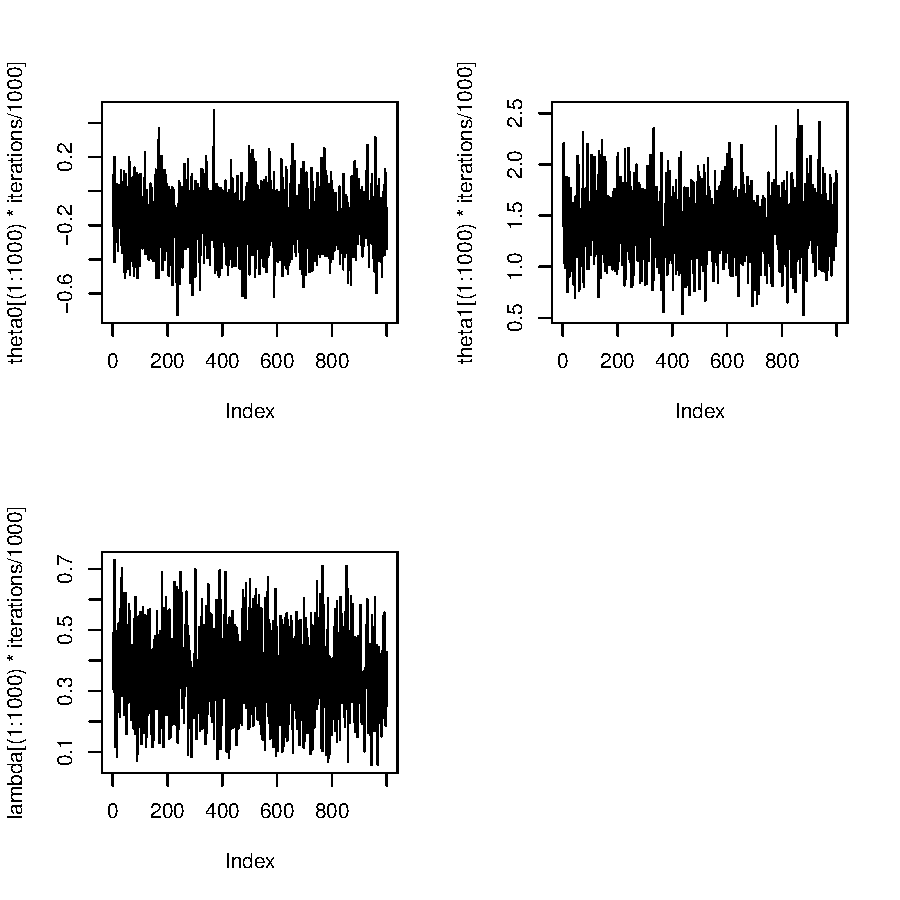
\includegraphics{takehomeSolutions2012-005}

These plots look great, so the number of iterations seems okay.  The only
question is how narrow our confidence intervals are and whether they 
give estimates that are precise enough for our purposes.  If not, we could
always use more iterations.
\end{quotation}

\item 
Give 95\% credible intervals for the two binomial 
proportions $\exp\{\theta_0\} / (1+\exp\{\theta_0\})$ and
$\exp\{\theta_1\} / (1+\exp\{\theta_1\})$.  Base these intervals
on the 0.025 and 0.975 quantiles of the $\theta_0$ and $\theta_1$
parameters, respectively.
\begin{quotation}{\bf Solution:}
\begin{Schunk}
\begin{Sinput}
> inverseLogit <- function(x) exp(x) / (1+exp(x))
> inverseLogit(quantile(theta0, c(.025, .975))) # p0 credible interval
\end{Sinput}
\begin{Soutput}
     2.5%     97.5% 
0.3695248 0.5382474 
\end{Soutput}
\begin{Sinput}
> inverseLogit(quantile(theta1, c(.025, .975))) # p1 credible interval
\end{Sinput}
\begin{Soutput}
     2.5%     97.5% 
0.6872755 0.8896077 
\end{Soutput}
\end{Schunk}
\end{quotation}

\item 
Based on your MCMC run, give estimates of the 
posterior means of $Z_6, \ldots, Z_{10}$ along with 
corresponding confidence intervals.
\begin{quotation}{\bf Solution:}
For this, we'll use the batch means idea with $b=n/1000$ and $a=1000$:
\begin{Schunk}
\begin{Sinput}
> phat <- colMeans(z6toz10)
> phat # These are the estimated posterior means
\end{Sinput}
\begin{Soutput}
[1] 0.0002369998 0.9973890026 0.1915768084 0.0031239969 0.0087559912
\end{Soutput}
\begin{Sinput}
> b <- iterations/1000
> a <- 1000
> varHat <- rep(0, 5)
> for (j in 1:5) {
+   y <- rowMeans(matrix(z6toz10[-1, j], nrow=b, byrow=TRUE))
+   varHat[j] <- b*var(y)
+ }
> lowerBounds <- phat - 1.96 * sqrt(varHat / iterations)
> upperBounds <- phat + 1.96 * sqrt(varHat / iterations)
> rbind(lowerBounds, upperBounds) # There are the conf intervals
\end{Sinput}
\begin{Soutput}
                    [,1]      [,2]      [,3]        [,4]        [,5]
lowerBounds 0.0001984312 0.9972802 0.1902892 0.002999160 0.008537393
upperBounds 0.0002755684 0.9974978 0.1928644 0.003248833 0.008974590
\end{Soutput}
\end{Schunk}

Interestingly, the posterior means leave little doubt about the
most likely classification of the four $X_i$ values 5, 18, 8, and 9.
Only 12 is somewhat in doubt, with a posterior mean 
(i.e., probability of coming from the $\theta_1$ distribution)
of around 19\%.
\end{quotation}

\end{enumerate}




\end{document}
